\section{Multiple Network Models}
\label{sec:ch5:multi}


Up to this point, you have studied network models which are useful for a single network. What do you do if you have multiple networks?

Let's imagine that you have a company with $45$ total employees. $10$ of these employees are company administrative executives (Adm.), $25$ of these employees are network machine learning experts (ML), and $10$ of these employees are marketing experts (Mar.). You study the social media habits of your employees on Facebook, Twitter, and Linkedin. For a given social networking site, an edge is said to exist between a pair of employees if they are connected on the social media site (by being friends, following one another, or being connected, respectively). As it turns out, individuals tend to most closely associate with the colleagues whom they work most closely: you might expect some sort of community structure to your network, wherein network machine learning experts are more connected with network machine learning experts, marketing experts are more connected with marketing experts, so on and so forth. What you will see below is that all of the networks appear to have the same community organization, though on Linkedin, we see that the administrative executives tend to be a little more connected than the other team members. This is reflected in the fact that there are more connections between Adm. members on Linkedin and other team members. To do this, we'll use a homophilic stochastic block model from Section \ref{sec:ch5:psd_block} for the Facebook and Twitter networks, and a homophilic degree-corrected stochastic block model (with $\theta = 1$ for non-Adm. team members, and $\theta=\sqrt 3$ for Adm. team members) for the Linkedin network. We will borrow the \texttt{dcsbm} function from Section \ref{sec:ch5:dcsbm}:

\begin{lstlisting}[style=python]
from graspologic.simulations import sbm
import numpy as np
from graphbook_code import dcsbm

K = 3
# between-community connection prob. is 0.05
B = 0.05*np.ones((K, K))
# homophilic connection prob. is 0.3
np.fill_diagonal(B, 0.3)

ns = [50, 25, 25]
theta = np.ones((np.sum(ns),1))
theta[ns[0]:(ns[0] + ns[1]),:] = np.sqrt(2)

# our dcsbm function only works with communities encoded 1,2,...,K
# so we will need to generate zs still
labels = ["ML" for i in range(ns[0])] + ["Adm." for i in range(ns[1])] + \
    ["Mar." for i in range(ns[2])]

z = np.array([1 for i in range(ns[0])] + [3 for i in range(ns[0])] + \
    [3 for i in range(ns[0])])
# sample the random networks, and use sbm() to generate zs for us
A_fb, zs = sbm(n=ns, p=B, return_labels=True)
A_tw = sbm(n=ns, p=B)
A_li, P_li = dcsbm(zs + 1, theta, B, return_prob=True)
\end{lstlisting}

We illustrate heatmaps from each of the three networks in Figure \ref{fig:ch5:socialnets}. Notice that while the Facebook and Twitter networks do not look particularly different, the Linkedin network appears to show that administrative members tend to have much higher numbers of connections with other members.

\begin{figure}[h]
    \centering
    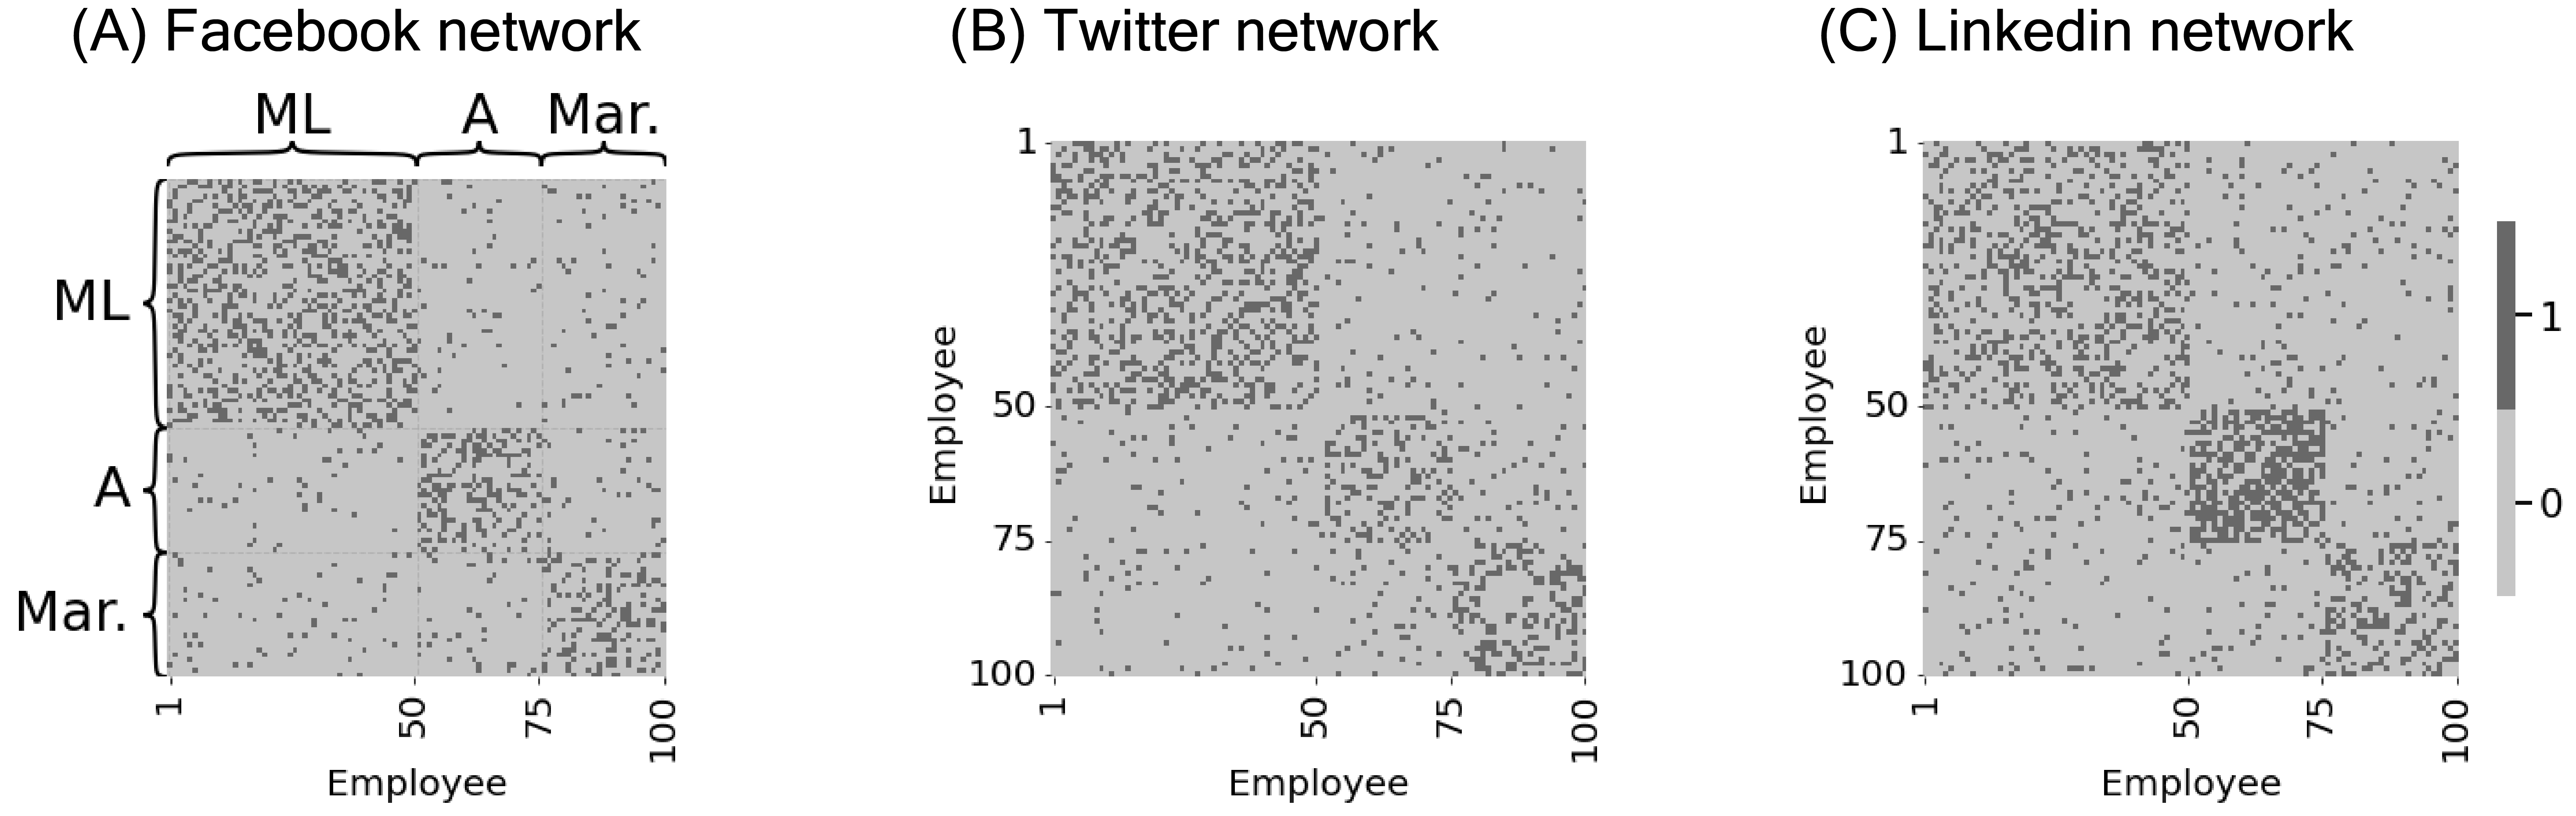
\includegraphics[width=\linewidth]{representations/ch5/Images/socialnets.png}
    \caption[Social networks for employees across Facebook, Twitter, and Linkedin.]{\textbf{(A)} Facebook social network. \textbf{(B)} Twitter social network. \textbf{(C)} Linkedin social network. Notice that on Linkedin, the administrators tend to have more edges.}
    \label{fig:ch5:socialnets}
\end{figure}

Remember that a random network has an adjacency matrix denoted by a boldfaced uppercase $\mathbf A$, and has network samples $A$ (which we just call "networks"). When you have multiple networks, you will need to be able to index them individually. For this reason, in this section, you will use the convention that a random network's adjacency matrix is denoted by a boldfaced uppercase $\mathbf A^{(m)}$, where $m$ tells you which network in your collection you are talking about. The capital letter $M$ defines the \textit{total} number of random networks in your collection. 

In your social network example, since you have connection networks for $3$ sites, $N$ is $3$. When you use the letter $m$ itself, you will typically be referring to an arbitrary random network among the collection of random networks, where $m$ is between $1$ and $N$. When we have $M$ total networks, we will write down the entire {collection of random networks} using the notation $\left\{\mathbf A^{(1)}, ..., \mathbf A^{(M)}\right\}$. With what you already know, for a random network $\mathbf A^{(m)}$, you would be able to use a single nework model to describe $\mathbf A^{(m)}$. This means, for instance, if you thought that each social network could be represented by a different RDPG, that you would have a {different} latent position matrix $X^{(m)}$ to define each of the $30$ networks. In symbols, you would write that each $\mathbf A^{(m)}$ is an RDPG random nework with latent position matrix $X^{(m)}$. What is the problem with this description?

What this description lacks is that the three networks share a {lot} of common information. You might expect that, on some level, the latent position matrices should also show some sort of common structure. This is because they each have the same block matrices, despite the fact that the Linkedin network incorporated a degree-correction factor for the administrative team.

However, since you used a {unique} latent position matrix $X^{(m)}$ for each random network $\mathbf A^{(m)}$, you have inherently stated that you think that the networks have distinct latent position matrices. If you were to perform a task downstream, such as whether you could identify which employees are in which community, you would have to analyze each latent position matrix individually, and you would not be able to learn a latent position matrix with shared structure across the three networks. Before you jump into multiple network models, let's provide some context as to how you will build these up.

In the below descriptions, we will tend to build off the Random Dot Product Graph (RDPG), and closely related variations of it. Why?

The reason for this is that as we have built up over several sections, the $RDPG_n(X)$ random networks can unify all positive semi-definite $IER_n(P)$ networks. This means that building off the RDPG gives you multiple random network models that will be inherently flexible. One of the models that we will discuss will build off the ``generalized'' RDPG, the gRDPG \cite{Rubin2022Sep,Arroyo2021} as well, which will allow us to generalize to arbitrary $IER_n(P)$ networks. Together, these models are extremely common across numerous disciplines of network machine learning, such as social networking, neuroscience, and many other fields.

So, how can you model your collection of random networks with shared structure?
\subsection{Joint Random Dot Product Graphs (JRDPG) Model}
\label{sec:ch5:multi:jrdpg}
In our example on social networks, notice that the Facebook and Twitter connections do not look {too} qualitatively different. It looks like they have relatively similar connectivity patterns between the different employee working groups, and you might even think that the underlying random network that governs these two social networks are {identical}. In statisical science, when we have a collection of $M$ random networks that have the same underlying random process, we describe this with the term {homogeneity}. Let's put what this means into context using your coin flip example. If a pair of coins are {homogeneous}, this means that the probability that they land on heads is identical. Likewise, this intuition extends directly to random networks. 

\subsubsection{Homogeneous and heterogeneous collections of random networks}
A \textit{homogeneous} collection of independent-edge random networks $\left\{\mathbf A^{(1)}, ..., \mathbf A^{(M)}\right\}$ is one in which {all} of the $M$ random networks have the {same probability matrix}, and consequently have the same distribution (statistically, the term is {identically distributed}). Remember that the probability matrix $P^{(m)}$ is the matrix whose entries $p^{(m)}_{ij}$ indicate the probability that an edge exists between nodes $i$ and $j$. This is because the probability matrix is the fundamental unit which can be used to describe independent-edge random networks, as we learned in Section \ref{sec:ch5:ier}. On the other hand, a \textit{heterogeneous} collection of independent-edge random networks is a collection of networks $\left\{\mathbf A^{(1)}, ..., \mathbf A^{(M)}\right\}$ is one in which the probability matrices are {not} the same for all of the $M$ networks, and hence, they are {not} identically distributed. 

The probability matrices $P^{(1)}$ and $P^{(2)}$ for the random networks $\mathbf A^{(1)}$ and $\mathbf A^{(2)}$ for Facebook and Twitter from the example we introduced above are identical, because they have the same community assignment vector and the same block matrix. Since the probability for an $SBM_n(\vec z, B)$ random network is only a function of these two things as we saw in Algorithm \ref{alg:ch5:sbm_pmtx}, the probability matrices are the same.

\subsubsection{Conceptualizing the $JRDPG_{n,M}(X)$ model}
The Joint Random Dot Product Graphs (JRDPG) is the simplest way you can extend the RDPG random network model to multiple random networks. The way you can think of the JRDPG model is that for each of your $M$ total random neworks, the edges depend on a latent position matrix $X$. We say that a collection of random networks $\left\{\mathbf A^{(1)}, ..., \mathbf A^{(N)}\right\}$ with $n$ nodes is $JRDPG_{n,M}(X)$ if each random network $\mathbf A^{(m)}$ is $RDPG_n(X)$ and if the $M$ networks are independent. The joint random dot product graph model is formally described by \cite{Athreya2017Jan}, and has many connections with the omnibus embedding \cite{Levin2017}, which you will learn about in Section \ref{sec:ch6:multinet}.

\subsubsection{The JRDPG model does not allow you to heterogeneity}

Under the JRDPG model, each of the $M$ random networks share the same latent position matrix. Remember that for an RDPG, the probability matrix $P = XX^\top$. This means that for all of the $M$ networks, $P^{(m)} = XX^\top$ under the JRDPG model. hence, $P^{(1)} = P^{(2)} = ... = P^{(M)}$, and {all} of the probability matrices are {identical}! This means that the $M$ random networks are {homogeneous}. Consequently, the JRDPG can be thought of as $M$ homogeneous and independent RDPGs.

From Section \ref{sec:ch5:ier:sbm_pmtx}, we learned how to construct probability matrices from homophilic block matrices. Let's try this by generating the latent position matrices, using the process that we outlined in Section \ref{sec:ch5:ier:sbm_pmtx}:

\begin{lstlisting}[style=python]
from graphbook_code import generate_sbm_pmtx

# we already returned P_li for the linkedin
# probability matrix from dcsbm() function
P_fb_tw = generate_sbm_pmtx(z, B)
# when plotting for comparison purposes, make sure you are
# using the same scale from 0 to 1
heatmap(P_fb_tw, vmin=0, vmax=1)
heatmap(P_li, vmin=0, vmax=1)
heatmap(P_li - P_fb_tw, vmin=0, vmax=1)
\end{lstlisting}

\begin{figure}[h]
    \centering
    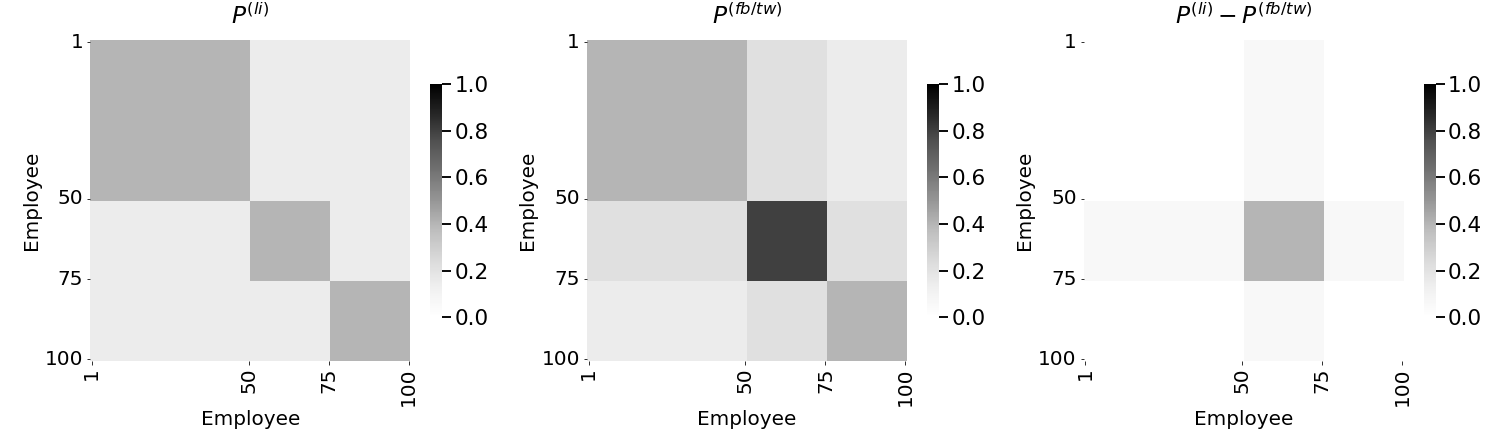
\includegraphics[width=\linewidth]{representations/ch5/Images/het.png}
    \caption[Heterogeneous random network probability matrices]{\textbf{(A)} the probability matrix for the random networks underlying twitter and facebook, $\mathbf A^{(1)}$ and $\mathbf A^{(2)}$. \textbf{(B)} the probability matrix for the random networks underlying linkedin. \textbf{(C)} the difference between the probability matrices for twitter/facebook and linkedin.}
    \label{fig:ch5:het}
\end{figure}
We illustrate heatmaps of the probability matrices in Figure \ref{fig:ch5:het}. Since the probability matrices for Facebook and Twitter in \ref{fig:ch5:het}(A) are exactly identical (they are both functions of the same community assignment vector $\vec z$ and block matrix $B$), the collection of random networks $\left\{\mathbf A^{(1)}, \mathbf A^{(2)}\right\}$ are homogeneous. You could model this pair of networks using the JRDPG due to their homogeneity and the fact that the underlying block matrices are homophilic (and hence, positive semi-definite with a positive semi-definite probability matrix).

On the other hand, $\mathbf A^{(1)}$ an $\mathbf A^{(2)}$ do not have the same probability matrix as $\mathbf A^{(3)}$, as shown in Figure \ref{fig:ch5:het}(B) and (C). This means that the collections of random networks $\left\{\mathbf A^{(1)}, \mathbf A^{(3)}\right\}$, $\left\{\mathbf A^{(2)}, \mathbf A^{(3)}\right\}$, and $\left\{\mathbf A^{(1)}, \mathbf A^{(2)}, \mathbf A^{(3)}\right\}$ are {heterogeneous}, because their probability matrices are different. 

So, unfortunately, the JRDPG cannot handle the hetereogeneity between the random networks of Facebook and Twitter with the random network for Linkedin. To remove this restrictive homogeneity property of the JRDPG, we can turn to a single network model that we just covered: the $IER_n(P)$ random network. Next, you will see how the IER random network can be used in conjunction with the COSIE model to allow you to capture this heterogeneity. 


\subsection{Common Subspace Independent Edge (COSIE) Model}
\label{sec:ch5:multi:cosie}

In our example on social networks, notice that the Facebook and Linkedin connections looked relatively similar, but had an important difference: on Linkedin, there was an administrative meeting, and the employees on the administrative team exchanged far more connections than usual among one another. It turns out that, in fact, the independent-edge random networks $\mathbf A^{(1)}$ and $\mathbf A^{(3)}$ which underly the social networks $A^{(1)}$ and $A^{(3)}$ were also different, because the probability matrices were different, which we explored in Figure \ref{fig:ch5:het}. 

This {heterogeneity} was driven by the members of the administrative teams having more connections with other nodes than members of the other teams in the Linkedin network (a degree-correction factor of $\sqrt 3$), despite the fact that there was shared structure (the block matrices underlying the $DCSBM_n(\vec z, \vec\theta, B)$ random network for Linkedin and the $SBM_n(\vec z, B)$ random networks for Facebook/Twitter were the same).

\subsubsection{The COSIE Model is defined by a collection of score matrices and a shared low-rank subspace}

Even though $P^{(1)}$ and $P^{(3)}$ are not {identical}, you can see they still share {some} structure: the employee teams are the same between the two social networks, and much of the probability matrix is unchanged. For this reason, it will be useful for you to have a network model which allows you to convey {some} shared structure, but still lets you convey aspects of the different networks which are {unique}. Ultimately, our goal with network modelling is to make sense of the networks we observe downstream, which is difficult to do when there are too many things you need to estimate or think about simultaneously. This {shared structure} will allow you to {borrow strength} when you estimate, which will allow you to feasibly estimate all of the ingredients you will need to describe COSIE networks. The COSIE model will accomplish this using a {shared latent position matrix} to describe the {similarities}, and unique {score matrices} to describe the {differences}, for each of the random networks. Let's learn about what these are.

\paragraph{The Shared Latent Position Matrix Describes Similarities}
\label{sec:ch5:multi:cosie:slpm}

The {shared latent position matrix} for the COSIE model is quite similar to the latent position matrix for an RDPG. Like the latent position matrix, the shared latent position matrix $V$ is a matrix with $n$ rows (one for each node) and $d$ columns. The $d$ columns behave very similarly to the $d$ columns for the latent position matrix of an RDPG, and $d$ is referred to as the \textit{latent dimensionality} of the COSIE random networks. Like before, each row of the shared latent position matrix $\vec v_i$ will denote the shared latent position vector for node $i$.

We will also add an additional restriction to $V$: it will be a matrix with orthonormal columns. What this means is that for each column of $V$, the dot product of the column with itself is $1$, and the dot product of the column with any other column is $0$. This has the implication that $V^\top V = I$, the identity matrix. All this has the effect of doing is it gives you a sense of uniform scale for all of the columns (scale $1$) of the latent position matrix. This has the effect of allowing the other component, the {score matrix}, to be interpretable, which you will learn more about in the next subsection.  

The shared latent position matrix conveys the {common structure} between the COSIE random networks, and will be a parameter for each of the neworks. Remember that with the $JRDPG_n(X)$ model, you were able to express the homogeneity of the social networks on Facebook and Twitter, but you could not capture the heterogeneity of the social nework on Linkedin. However, you want the shared latent position matrix $V$ to convey the commonality among the three social networks; that is, that the employees are always working on the same employee teams. 

Unfortunately, obtaining these latent position matrices analytically is difficult. For this reason, we will use the probability matrix combined with a later method that we describe in Section \ref{sec:ch6:multinet}, called \texttt{MASE}, to obtain them for us so that we can explain the core logic of the model. For now, we will ignore this technique, and circle back to it later on. First, let's use \texttt{MASE} to obtain the shared latent positions:

\begin{lstlisting}[style=python]
from graspologic.embed import MultipleASE as MASE
from graphbook_code import lpm_heatmap

embedder = MASE(n_components=3)
# obtain shared latent positions
V = embedder.fit_transform([P_fb_tw, P_fb_tw, P_li])

lpm_heatmap(V)
\end{lstlisting}

The shared latent position matrix is shown in Figure \ref{fig:ch5:het}(A). This matrix is arranged exactly as you are accustomed to from Section \ref{sec:ch5:rdpg} on the $RDPG_n(X)$ random network, and is interpreted similarly: the rows indicate nodes (employees), and the columns indicate latent dimensions. Each row of $V$ indicates the latent position of a given node $i$.

One thing should immediately jump out to you: the latent positions are the {same} for all employees across a given community assignment (their role in the company). This makes perfect sense based on what we learned from Section \ref{sec:ch5:psd_block:same_lp}. You should go re-read that section, because we are about to draw heavily from it.

The Facebook and Twitter examples were just $SBM_n(\vec z, B)$ random networks with a homophilic block matrix, so the latent positions should be identical across all nodes from a given community. Also, for the Linkedin example, the degree-correction factors were identical within each community, so it also makes sense that the latent positions should be identical across all nodes from a given community there, too.

The COSIE model has taken this a step further: the homophilic (and hence, positive semi-definite) block matrix $B$ itself is identical across all of the networks, which means that for each network, a node $i$ in community $1$ would have the latent position:
\begin{align*}
    \vec x_i^{(1)}^\top = \vec x_i^{(2)}^\top = \begin{bmatrix}1 & 0 & 0\end{bmatrix} \sqrt B
\end{align*}
for Facebook and Twitter, and for Linkedin, is:
\begin{align*}
    \vec x_i^{(3)}^\top = \theta_i\begin{bmatrix}1 & 0 & 0\end{bmatrix} \sqrt B
\end{align*}
Notice, in particular, that $\vec x_i^{(3)}$ is equivalent to $\vec x_i^{(1)}$ and $\vec x_i^{(2)}$, up to the rescaling by $\theta_i$ (the degree-correction factor). You could repeat this for all of the communities to deduce that the shared latent positions for the Linkedin network should just be a rescaling of the shared latent positions from the Facebook and Twitter networks.

Looking at the shared latent position matrix, the COSIE model can capture what we already know: there is a strong degree of {homogeneity} across the different networks; the latent positions are identical (up to a rescaling) and, in fact, you can represent them with the same shared latent position matrix. 

Now, what about the unique aspects; particularly, that $\theta_i$ term, for the administrative team?

\paragraph{Score Matrices Describe Differences}
\label{sec:ch5:multi:cosie:score}

The \textit{score matrices} for the COSIE random networks essentially tell you how to assemble the shared latent position matrix to obtain the unique probability matrix for each network. The score matrix $R^{(m)}$ for a random network $m$ is a matrix with $d$ columns and $d$ rows. Therefore, it is a square matrix whose number of dimensions is equal to the latent dimensionality of the COSIE random networks.

The probability matrix for each network under the COSIE model is the matrix:
\begin{align*}
    P^{(m)} &= VR^{(m)}V^\top
\end{align*}
When we look at this expression, we can understand it a little bit better by focusing on the first multiplication, the term $VR^{(m)}$. You are basically taking the shared latent position matrix, and using the scores to express which latent position vectors are more, or less, important in the probability matrix $P^{(m)}$. In this sense, the score matrix tells you which combinations of latent positions determine the unique features of heterogeneous probability matrices.

In the social network example, we want the score matrices to indicate that Facebook and Twitter share a probability matrix, but Facebook and Linkedin do not. Consequently, we would expect that the score matrices from Facebook and Twitter should be the same, but the score matrix for Linkedin will be different. We can obtain these with the \texttt{MASE} object, which again, isn't too important to understand perfectly just yet:

\begin{lstlisting}[style=python]
# obtain score matrices
R_fb = embedder.scores_[0,:,:]
R_tw = embedder.scores_[1,:,:]
R_li = embedder.scores_[2,:,:]

# and plot them
smin = np.min(embedder.scores_); smax = np.max(embedder.scores_)
fig, axs = plt.subplots(1, 3, figsize=(20, 7))
heatmap(R_fb, vmin=smin, vmax=smax)
heatmap(R_tw, vmin=smin, vmax=smax)
heatmap(R_li, vmin=smin, vmax=smax)
\end{lstlisting}
We plot the score matrices in Figure \ref{fig:ch5:scores}. As you can see from the plot, the score matrices for Facebook and Twitter are identical, but the score matrix for Linkedin is distinct.

\begin{figure}
    \centering
    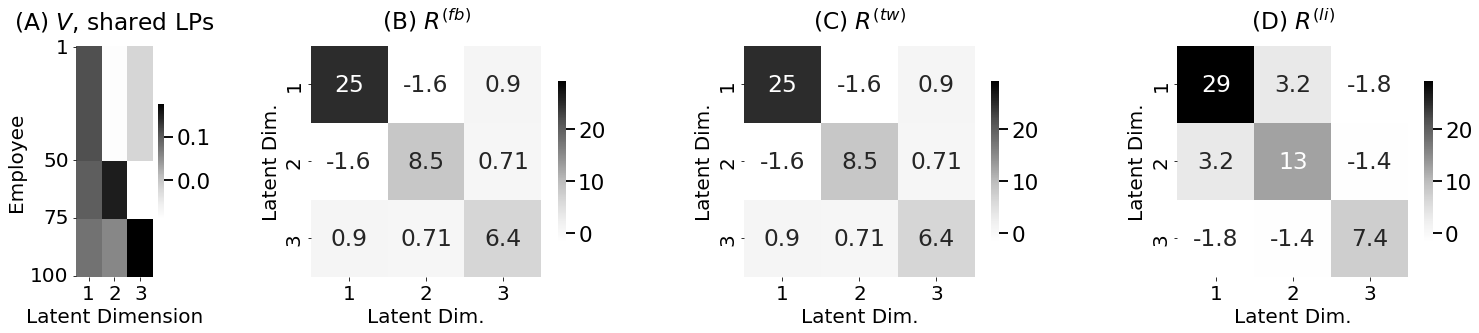
\includegraphics[width=\linewidth]{representations/ch5/Images/scores.png}
    \caption[Score matrices for COSIE model]{\textbf{(A)} the shared latent position matrix across all of the networks. \textbf{(B)} score matrix for the Facebook random network. \textbf{(C)} score matrix for the Twitter random network. \textbf{(D)} score matrix for the Linkedin random network.}
    \label{fig:ch5:scores}
\end{figure}

\subsubsection{Conceptualizing the COSIE model}

Finally, let's relate all of this back to the COSIE model. The way you can think about the COSIE model is that for each random network that you have, the probability matrix $P^{((m)}$ depends on the shared latent position matrix $V$ and the score matrix $R^{(m)}$. The probability matrix $P^{(m)}$ for the $m^{th}$ random network is defined so that $P^{(m)} = VR^{(m)}V^\top$. This means that each entry $p_{ij}^{(m)} = \vec v_i^\top R^{(m)} \vec v_j$. We say that a collection of random networks $\left\{\mathbf A^{(1)}, ..., \mathbf A^{(M)}\right\}$ with $n$ nodes is $COSIE_{n,M}\left(V, \left\{R^{(1)},...,R^{(M)}\right\}\right)$ if each random network $\mathbf A^{(m)}$ is $IER(P^{(m)})$. Stated another way, each of the $M$ random networks share the same orthonormal matrix $V$, but a unique score matrix $R^{(m)}$. This allows the random networks to share some underlying structure (which is conveyed by $V$) but each random network still has a combination of this shared structure (conveyed by $R^{(m)}$). 

Since the probability matrix $P^{(m)} = VR^{(m)}V^\top$, you can see that two random networks with the same score matrix will be homogeneous (identically distributed), and two random networks with different score matrices will be heterogeneous (not identically distributed). In this way, you are able to capture the homogeneity between the random networks for Facebook and Twitter connections, while also capturing the heterogeneity between the random networks for Facebook and Linkedin connections. The COSIE model is described by \cite{Arroyo2021}, and has direct connections with the multiple adjacency spectral embedding, which you will learn about in Section \ref{sec:ch6:multinet}.

\begin{floatingbox}[h]\caption{Check what you've learned}
To double check what you've learned so far, we would recommend that you play around with these results some. 

Demonstrate that you are able to recover the using the shared latent position matrices \texttt{V} and the score matrices \texttt{R\_fb}, \texttt{R\_tw}, and \texttt{R\_li}. 

Show that the true probability matrices \texttt{P\_fb\_tw} and \texttt{P\_li} are identical to the probability matrices that you obtain using the shared latent positions and the score matrices by using \texttt{np.allclose()}, like we did in Section \ref{sec:ch5:psd_block:lpm_fromsbm}.
\end{floatingbox}

\paragraph{Connections with the gRDPG}

The gRDPG random network, introduced briefly in Section \ref{sec:ch5:ier:grdpg}, is a little bit tough to conceptualize. To be precise, the initial formulation of the COSIE model in \cite{Arroyo2021} describes random networks which are gRDPGs (a broad class of models that is equivalent to IERs). To this end, the distinction is merely one of convenience for the audience: for expert statisticians who have built their careers in random network theory, the gRDPG may be more straightforward; to a broader audience, IER might be more straightforward. 

\subsection{Correlated Network Models}
\label{sec:ch5:multi:corr}

Finally, we get to a special case of network models, known as correlated network models. Let's say that you have a group of people in a city, and you know that each person in your group have both a Facebook and a Twitter account. The nodes in your network are the people who possess accounts. The first network consists of Facebook connections among the people, where an edge exists between two people if they are friends on Facebook. The second network consists of Twitter connections among the people, where an edge exists between two people if they follow one another on Twitter. You think that if two people are friends on Facebook, there is a good chance that they follow one another on Twitter, and vice versa. How do you reflect this similarity through a multiple network model?

At a high level, network correlation between a pair of networks describes the property that the existence of edges in one network provides you with some level of information about edges in the other network, much like the Facebook/Twitter example that you just saw. In this book, we will focus on the $\rho$-{correlated} network models. What the $\rho$-correlated network models focus on is that given two random networks with the same number of nodes, each edge has a correlation of $\rho$ between the two networks. To define this a little more rigorously, a pair of random networks $\mathbf A^{(1)}$ and $\mathbf A^{(2)}$ are called $\rho$-\textbf{correlated} if all of the edges across both networks are mutually independent, except that for all pairs of indices $i$ and $j$, $corr(\mathbf a_{ij}^{(1)}, \mathbf a_{ij}^{(2)}) = \rho$, where $corr(\mathbf x, \mathbf y)$ is the Pearson correlation between two random variables $\mathbf x$ and $\mathbf y$. In our example, this means that whether two people are friends on Facebook is {correlated} with whether they are following one another on Twitter.

The Pearson correlation describes whether one variable being large/small gives information that the other variable is large/small (positive correlation, between $0$ and $1$) or whether one variable being large/small gives information that the other variable will be small/large (negative correlation, between $-1$ and $0$). If the two networks are positively correlated and you know that one of the edges $\mathbf a_{ij}^{(1)}$ has a value of one, then you have information that $\mathbf a_{ij}^{(2)}$ might also be one, and vice-versa for taking values of zero. If the two networks are negatively correlated and you know that one of the edges $\mathbf a_{ij}^{(1)}$ has a value of one, then you have information that $\mathbf a_{ij}^{(2)}$ might be zero, and vice-versa. If the two networks are not correlated ($\rho = 0$) you do not learn anything about edges of network two by looking at edges from network one.

\subsubsection{$\rho$-Correlated RDPG}
\label{sec:ch5:multi:corr:rrdpg}

The $\rho$-correlated RDPG is the most general correlated network model you will need for the purposes of this book, and is described by \cite{Lyzinski2014Jan} and \cite{Pantazis2022}. Remembering that both ER, SBM, and DCSBM random networks are special cases of the RDPG (as long as the block matrix is positive semi-definite), the $\rho$-correlated RDPG can therefore be used to construct $\rho$-correlated ER, $\rho$-correlated SBMs, and $\rho$-correlated DCSBMs too. The way you can think about the $\rho$-correlated RDPG is that like for the normal RDPG, a latent position matrix $X$ with $n$ rows and a latent dimensionality of $d$ is used to define the edge-existence probabilities for the networks $\mathbf A^{(1)}$ and $\mathbf A^{(2)}$. 

We begin by defining that $\mathbf A^{(1)}$ is $RDPG_n(X)$. Next, we define the second network as follows. We use a coin for each edge $(i, j)$, which has a probability that depends on the values that the first network takes. If the edge $\mathbf a_{ij}^{(1)}$ takes the value of one, then we use a coin which has a probability of landing on heads of $\vec x_i^\top \vec x_j + \rho(1 - \vec x_i^\top \vec x_j)$. If the edge $\mathbf a_{ij}^{(1)}$ takes the value of zero, then we use a coin which has a probability of landing on heads of $(1 - \rho)\vec x_i^\top \vec x_j$. We flip this coin, and if it lands on heads, then the edge $\mathbf a_{ij}^{(2)}$ takes the value of one. If it lands on tails, then the edge $\mathbf a_{ij}^{(2)}$ takes the value of zero. If $\mathbf A^{(1)}$ and $\mathbf A^{(2)}$ are random networks which are $\rho$-correlated RDPGs with latent position matrix $X$, we say that the pair $\left\{\mathbf A^{(1)}, \mathbf A^{(2)}\right\}$ are $\rho-RDPG_n(X)$. 


\subsection{How do you simulate samples of $SBM_n(\vec z, B)$ random networks?}

The procedure in Algorithm \ref{alg:ch5:rhordpg} will produce for you a pair of networks $A^{(1)}$ and $A^{(2)}$, which have nodes and edges, where the underlying random networks $\mathbf A^{(1)}$ and $\mathbf A^{(2)}$ are $\rho-RDPG_n(X)$ random networks.

\begin{algorithm}[h]\caption{Simulating a paired sample of $\rho RDPG(X)$ random networks}
\label{alg:ch5:rhordpg}
\SetAlgoLined
\KwData{$n$ a number of nodes\newline $X$ a latent position matrix with $n$ rows and $d$ columns \newline $\rho$ a correlation between the two networks that is between $-1$ and $1$}
\KwResult{A pair of random networks which are $\rho$-correlated.}

Simulate a sample $A^{(1)}$ which is a sample  of an $RDPG_n(X)$ random network, using Algorithm \ref{alg:ch5:rdpg}.

\For{$i$ in $1$:$n$} {
    \For{$j > i$} {
        \If{$a_{ij}^{(1)} = 1$}{
            Obtain a coin which has a probability of landing on heads of $\vec x_i^\top \vec x_j + \rho(1 - \vec x_i^\top \vec x_j)$.
        } \Else {
            Obtain a coin which has a probability of landing on heads of $(1 - \rho)\vec x_i^\top \vec x_j$.
        }
        
        Flip the coin, and if it lands on heads, the corresponding entry $a_{ij}^{(2)}$ in the adjacency matrix is $1$. If the coin lands on tails, the corresponding entry $a_{ij}^{(2)}$ is $0$. 

        Set $a_{ji}^{(2)} = a_{ij}^{(2)}$.
    }
}

\Return{$A^{(1)}$ and $A^{(2)}$}

\end{algorithm}


Fortunately, \texttt{graspologic} makes sampling $\rho$-correlated RDPGs relatively simple. Let's take the same underlying model that we were working with above, and assert that the networks are not only identical in probability, but that they are also {correlated}. 

Conceptually, this is similar to asserting that if we knew that a pair of people were friends on Facebook, we might think that they would be more likely to be following one another on Twitter. We'll start by generating latent position matrices corresponding to the Twitter/Facebook example using code from Section \ref{sec:ch5:psd_block:lpm_fromsbm}:
\begin{lstlisting}[style=python]
from graphbook_code import lpm_from_sbm

X_fb_tw = lpm_from_sbm(zs + 1, B)
\end{lstlisting}

Let's see what happens when the underlying correlation is $\rho = 0.7$. To summarize the differences between the two networks, we'll count the total number of edges that differ between the two networks, $\texttt{diff}\left(A^{(1)} - A^{(2)}\right)$:

\begin{lstlisting}[style=python]
from graspologic.simulations import rdpg_corr

# generate the network samples
rho = 0.7
A_fb_corr, A_tw_corr = rdpg_corr(X_fb_tw, Y=None, r=rho)

# the difference matrix
diff_mtx_corr = np.abs(A_fb_corr - A_tw_corr)
# the total number of differences
diff_fb_tw_corr = diff_mtx.sum()
\end{lstlisting}

A heatmap of the two networks is shown in Figure \ref{fig:ch5:rhordpg}(A) and Figure (B), along with the difference matrix in Figure \ref{fig:ch5:rhordpg}(C).

\begin{figure}
    \centering
    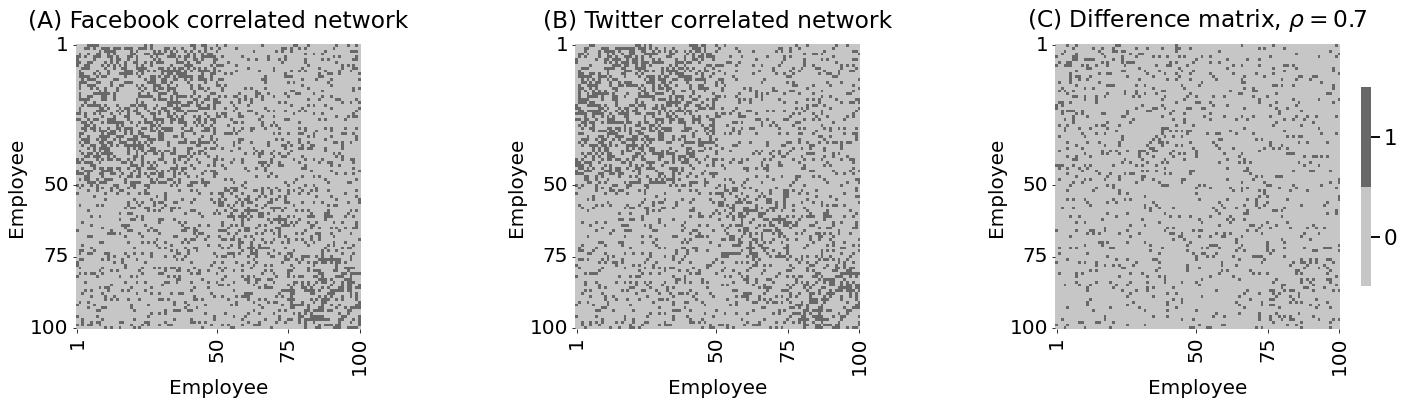
\includegraphics[width=\linewidth]{representations/ch5/Images/rhordpg.png}
    \caption[$\rho$-correlated RDPGs]{\textbf{(A)} the Facebook network. \textbf{(B)} the Twitter network. \textbf{(C)} the edges which differ between the two networks.}
    \label{fig:ch5:rhordpg}
\end{figure}
When the underlying correlation is much lower, such as $\rho' = 0.0$ (the networks are \textit{uncorrelated}), we can do the exact same thing:

\begin{lstlisting}[style=python]
rho_nil = 0.0
A_fb_nocorr, A_tw_nocorr = rdpg_corr(X_fb_tw, Y=None, r=rho_nil)

# the difference matrix
diff_mtx_nocorr = np.abs(A_fb_nocorr - A_tw_nocorr)
# the total number of differences
diff_fb_tw_nocorr = diff_mtx_nocorr.sum()
\end{lstlisting}

A heatmap of the two networks is shown in Figure \ref{fig:ch5:norhordpg}(A) and Figure (B), along with the difference matrix in Figure \ref{fig:ch5:norhordpg}(C). In both \ref{fig:ch5:rhordpg} and \ref{fig:ch5:norhordpg}, the Facebook and Twitter networks have {identical} latent position matrices, and the latent position matrices are the same for both scenarios. However, when the networks are correlated, the edges tend to be more similar between the two networks. When the networks are uncorrelated, the edges tend to differ more between the two networks. 

\begin{figure}[h]
    \centering
    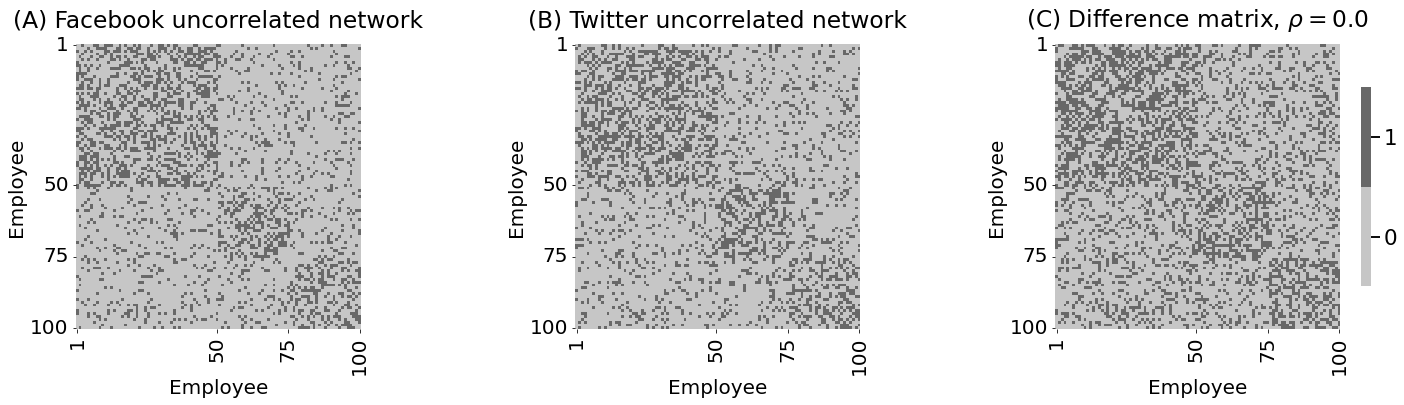
\includegraphics[width=\linewidth]{representations/ch5/Images/norhordpg.png}
    \caption[Uncorrelated RDPGs]{\textbf{(A)} the Facebook network. \textbf{(B)} the Twitter network. \textbf{(C)} the edges which differ between the two networks. Note that there are far more edges that differ than in Figure \ref{fig:ch5:rhordpg}.}
    \label{fig:ch5:norhordpg}
\end{figure}

\begin{floatingbox}[h]\caption{Negative $\rho$-correlated RDPGs}
If we generated another simulation where the networks were anti-correlated, we could arbitrarily increase the magnitude of this difference. Try the simulation again with $\rho$ as large as $-1$, and describe what you see. Repeat it a few times, and describe your result.

Next, do the simulation again with $\rho = 1.0$. What do you notice?
\end{floatingbox}

\newpage